\documentclass[12pt]{article}
\usepackage[a4paper,margin=2.2cm]{geometry}
\usepackage{amsmath,amssymb,amsthm,mathtools}
\usepackage{hyperref}
\usepackage{cleveref}
\usepackage{tikz}
\usetikzlibrary{arrows.meta,angles,quotes}



% 中文（xelatex）
\usepackage{fontspec}
\usepackage{xeCJK}
\setCJKmainfont{Noto Serif CJK SC}

\title{Linear Algebra}
\date{}
\begin{document}
\maketitle

首先我们要弄明白点积是什么
以 
1: $\vec{u} = \begin{bmatrix}
    1 \\
    2
\end{bmatrix}, \vec{v} = \begin{bmatrix}
    3 \\
    4
\end{bmatrix} $
为分析对象

\begin{center}
\begin{tikzpicture}[>=Stealth]
  \coordinate (O) at (0,0);
  \coordinate (U) at (1,2);
  \coordinate (V) at (3,4);

  \draw[->] (-0.2,0) -- (5.5,0) node[right] {$x$};
  \draw[->] (0,-0.2) -- (0,5.5) node[above] {$y$};

  \draw[->,thick] (O) -- (U) node[above left] {$\vec u=(1,2)$};
  \draw[->,thick] (O) -- (V) node[above right] {$\vec v=(3,4)$};

  % 夹角：U--O--V 表示在 O 点，射线 OU 到 OV 的角
  \pic[draw,->,"$\theta$", angle radius=1.2cm, angle eccentricity=1.25]
    {angle = V--O--U};
\end{tikzpicture}
\end{center}

\begin{flushleft}
点积的结果是一个值
它的几何公式是 
\[
\mathbf u \cdot \mathbf v = \|\mathbf u\|\,\|\mathbf v\|\cos\theta
\]

上图:
U = $\|u\|$  V = $\|v\|$ \\
那么 $V \cdot \cos\theta$ 表现的是什么？\\
$\cos\theta$ 是夹角 由直角三角形定理 $\cos\theta=\frac{邻边}{斜边}$\\
那么存在三个特殊的值 \\

当 $\cos\theta$ =  $90\textdegree$ 时  $cos\theta$ = 0 (点 p(0,y)) \\ 
当 $\cos\theta$ =  $180\textdegree$ 时 $cos\theta$ = -1(点 p(-x, 0)) \\ 
当 $\cos\theta$ =  $270\textdegree$ 时 $cos\theta$ = 0(点 p(0, -y)) \\ 
当 $\cos\theta$ =  $360\textdegree$ 或 $0\textdagger$ 时 $cos\theta$ = 1(点 p(x, 0)) \\ 

在标准圆中概念: 所有圆弧的点到(0,0) 都是相等的 等于1 \\ 
那么 $\cos\theta$ 就是一个带符号(方向)的比例值 \\ 
这是由角度转换称比例的思想  \\ 
那么我们就能解释 $V \cdot \cos\theta$ 是什么意思？它就是 V 的 子段长度 可能并不重合(因为带方向) \\ 

现在我们并不知道 $\cos\theta$ 的具体值,但我们知道 U 和 V \\  
那么 $\cos\theta = U / V$   \\ 
那么我们就可以得出   \\ 
$V \cdot \cos\theta$ 是 V 在 U 上的映射 \\ 
\[
\mathbf u \cdot \mathbf v = \|\mathbf u\|\,\|\mathbf v\|\cos\theta
\]
那么 V * (V 在 U 上的映射) 是 乘法的数学特性 \\ 
"趋势" 通常是使用 乘法 而非加法  \\ 

所以我们得出下面概念 \\ 
点积是趋势的一种表达(两个向量的相似度) \\ 

那么为什么点积的代数公式是: \\ 
$\vec{u} * \vec{v} = x1\cdot x2 + y2\cdot y2$ \\ 
我们知道一个向量是首尾相连的 \\ 
以 $i = (1, 0),j = (0, 1)$的标准基向量 \\
$\vec{u} = ix1 + jy1$ \\
那么 $\vec{u} \cdot \vec{v}$ 
= $(ix1 + jy1) \cdot (ix2 + jy2) $
= $ix1 \cdot ix2 +  ix1 \cdot jy2 + jy1 \cdot ix2  +  jy1\cdot jy2$
= $x1x2i^{2}  + x1x2ij +  y1x2ij + y1y2j^{2}$
i * j = 0
i * i = 1
= $x1x2 + y1y2$

那么我们会得到一个值 $x1x2 + y1y2$ 这个值就可以用于对比趋势 a-b 越小 两个相似度越近
\end{flushleft}

\section*{Q1.计算}
计算下列向量的的点积 $\vec{u} \cdot \vec{v}$

1. $\vec{u} = \begin{bmatrix}
    1 \\ 
    2
\end{bmatrix} ,\vec{v} = \begin{bmatrix}
    3 \\ 
    4
\end{bmatrix}  $

= 1*3  + 4*2  =  11

2. $\vec{u} = \begin{bmatrix}
    2 \\ 
    2
\end{bmatrix} ,\vec{v} = \begin{bmatrix}
    1 \\ 
    -1
\end{bmatrix}  $

=  2 + (-2) = 0


\section*{Q2.Angle Detection}
= $\cos \theta$ = 6/6 \\ 
= 1 \\ 


\section*{Q3.Normalization}
1.将 $\vec{v} = \begin{bmatrix}
    3\\
    4
\end{bmatrix}$
= $\begin{bmatrix}
    3 / \sqrt{3^{2} + 4^{2}} \\
    4 / \sqrt{3^{2} + 4^{2}}
\end{bmatrix}$

= $\begin{bmatrix}
    3 / 5 \\
    4 / 5
\end{bmatrix}$




\begin{flushleft}
\section*{Reboot}
    向量 $\vec{v}  =  \begin{bmatrix}
    x \\ 
    y
\end{bmatrix}$ \\
在标准X基准: \\  
$\vec{i}  =  \begin{bmatrix}
    1 \\ 
    0
\end{bmatrix}$,
在标准Y基准:  
$\vec{y}  =  \begin{bmatrix}
    0 \\ 
    1
\end{bmatrix}$ \\

的运动轨迹是
$\vec{v} = \vec{i} \cdot x  +  \vec{j} \cdot y $ \\ 

现在 $\vec{i}$ 变化到了一个新的位置  : $\vec{a} = \begin{bmatrix}
    2\\
    1
\end{bmatrix}$ \\ 
现在 $\vec{j}$ 变化到了一个新的位置  : $\vec{b} = \begin{bmatrix}
    -1\\
    0
\end{bmatrix}$ \\ 


那么问题: 在新的空间里 这个向量$\vec{v}$ 变成什么样了?
$\vec{v}_{new}$
= $\vec{a} \cdot x  +  \vec{b} \cdot y $ \\ 
= $\begin{bmatrix}
    2 \\
    1
\end{bmatrix} \cdot x  +  \begin{bmatrix}
    -1 \\
    0
\end{bmatrix}  \cdot y$
=  $\begin{bmatrix}
    2x \\
    1x
\end{bmatrix} +  \begin{bmatrix}
    -1y \\
    0y
\end{bmatrix} $
= $\begin{bmatrix}
    2x + (-1y) \\ 
    1x + 0y 
\end{bmatrix}
$
= $\begin{bmatrix}
    2x - y \\
    x 
\end{bmatrix}$ \\

我们从标准的  $\vec{v} = \vec{i} \cdot x  +  \vec{j} \cdot y $ \\ 
推理到 $\begin{bmatrix}
    2x + (-1y) \\ 
    1x + 0y 
\end{bmatrix}
$ 标准的行 * 列 \\
那么我们能不能把 $\vec{a}$ 和 $\vec{b}$ 合并起来呢 ?
我们先不考虑 $\vec{a}$ 和 $\vec{b}$ 合并起来的问题
我们先考虑 向量的行为 在 $\vec{i} \cdot x  +  \vec{j} \cdot y$的模型中
是典型的路线模型 -> 先按 $\vec{i}$ 规则 走 x步, 再按 $\vec{j}$ 规则走y步 \\ 
这个x,y 并不是坐标 而是数量,这点很重要 
当 $\vec{i}  =  \begin{bmatrix}
    1 \\ 
    0
\end{bmatrix}$, $\vec{y}  =  \begin{bmatrix}
    0 \\ 
    1
\end{bmatrix}$ \\
规则是标准坐标系

所以 $\vec{a} \cdot x  +  \vec{b} \cdot y $ \\ 
其实隐藏了 i 和 j 
所以 $\vec{a} \cdot (x \cdot \vec{i})  +  \vec{b} \cdot (y \cdot \vec{j}) $ \\ 
只不过 i 和 j 并不会对 x,y 产生任何变化
但从行为理解就很不一样：
从标准坐标系(环境) 以新的规则按先后到达新的地址
这个新的规则改变的是环境 
\end{flushleft}

\begin{flushleft}
\section*{Composition of Maps}

$\vec{x} = \begin{bmatrix}
    x \\
    y
\end{bmatrix}$ \\
矩阵 B: 
$B  = \begin{bmatrix}
    0 & 1 \\
    1 & 0
\end{bmatrix}$ \\
矩阵 A: 
$ A  = \begin{bmatrix}
    2 & 0 \\
    0 & 2 \\
\end{bmatrix}$ \\

计算： A @ (B @ x) 
= A @ $\begin{bmatrix}
    0x + 1y \\
    1x + 0y
\end{bmatrix}$ \\
= A @ $\begin{bmatrix}
    y \\
    x
\end{bmatrix}$ \\
= $\begin{bmatrix}
    2y + 0x \\
    0y + 2x
\end{bmatrix}$ \\
= $\begin{bmatrix}
    2y \\
    2x
\end{bmatrix}$ \\

A @ B 是否能执行？
如果 A B 的中间维度相同则存在意义 ((m * n) (n * k))

A @ B (使用标准的行*列运算)
= $\begin{bmatrix}
    2 & 0\\
    0 & 2
\end{bmatrix}$  @ 
$\begin{bmatrix}
    0 & 1 \\
    1 & 0
\end{bmatrix}$ \\
$ [0, 0] = 2 \cdot 0  + 0 \cdot 1 = 0 $ \\
$ [0, 1] = 2 \cdot 1  + 0 \cdot 0 = 2 $ \\
$ [1, 0] = 0 \cdot 0  + 2 \cdot 1 = 2 $ \\
$ [1, 1] = 0 \cdot 1  + 2 \cdot 0 = 0 $ \\
C = $\begin{bmatrix}
    0 & 2 \\
    2 & 0
\end{bmatrix}$ \\
= C @ x  \\
= $\begin{bmatrix}
    0x + 2y \\
    2x + 0y 
\end{bmatrix}$ \\
= $\begin{bmatrix}
    2y \\
    2x 
\end{bmatrix}$ \\
\end{flushleft}



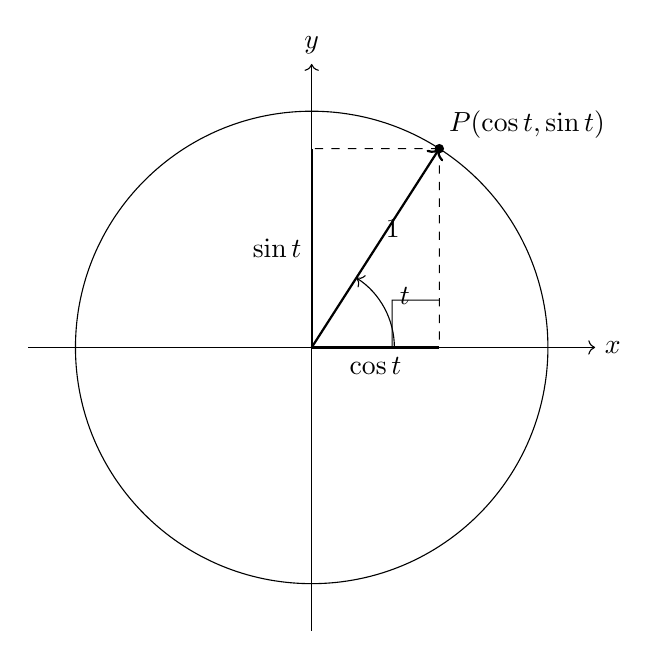
\begin{tikzpicture}[scale=3]

  % ====== 1) 设定角 t（弧度） ======
  \pgfmathsetmacro{\t}{1.0}        % 这里填弧度，比如 1.0 rad
  \pgfmathsetmacro{\ang}{deg(\t)}  % 转成角度给 TikZ 用

  % ====== 2) 坐标与点 ======
  \coordinate (O) at (0,0);
  \coordinate (P) at (\ang:1);      % 单位圆上点 P = (cos t, sin t)
  \coordinate (X) at (P |- O);      % (cos t, 0)
  \coordinate (Y) at (P -| O);      % (0, sin t)

  % ====== 3) 坐标轴 ======
  \draw[->] (-1.2,0) -- (1.2,0) node[right] {$x$};
  \draw[->] (0,-1.2) -- (0,1.2) node[above] {$y$};

  % ====== 4) 单位圆 ======
  \draw (O) circle (1);

  % ====== 5) 半径向量与点标注 ======
  \draw[->, thick] (O) -- (P) node[midway, above right] {$1$};
  \fill (P) circle (0.02) node[above right] {$P(\cos t,\sin t)$};

  % ====== 6) 投影虚线 ======
  \draw[dashed] (P) -- (X);
  \draw[dashed] (P) -- (Y);

  % ====== 7) 标出 cos t 与 sin t（作为“坐标/投影长度”） ======
  \draw[thick] (O) -- (X) node[midway, below] {$\cos t$};
  \draw[thick] (O) -- (Y) node[midway, left]  {$\sin t$};

  % ====== 8) 角 t 的弧（从 x 正轴转到 OP） ======
  \draw[->] (0.35,0) arc (0:\ang:0.35);
  \node at ({0.45*cos(\ang/2)},{0.45*sin(\ang/2)}) {$t$};

  % ====== 9) 直角标记（投影形成的直角） ======
  \draw pic[draw, angle radius=6mm] {right angle = P--X--O};

\end{tikzpicture}

\begin{flushleft}
\section{Inverse Matrix}
我们要弄清楚什么叫逆矩阵,
逆矩阵是一个矩阵, 所以它也是一种变换动作 \\
For example:

$\vec{y} = M @ \vec{x}$ \\
如果M 可逆 $-> M^{-1}$ \\ 
那么  
$\vec{x} = M^{-1} @ \vec{y}$ \\ 
那么我们推导出下面公式 \\ 
$\vec{x} = M^{-1} @ M  @ \vec{x}$ \\ 
= $M^{-1} @ M  = \begin{bmatrix}
    1 & 0 \\
    0 & 1
\end{bmatrix}$ ?(我不确定)

一个矩阵是否可逆根据是行列式决定  \\
那么我们首先要弄清楚行列式是什么： \\
$\vec{M} = \begin{bmatrix}
    a  &  b  \\
    c  &  d  
\end{bmatrix}$
行列式的公式 =  ad - bc

我们知道一个矩阵是可以被分解称两个基向量的模式 \\
$\vec{M}$ : \\
$ Mi = \begin{bmatrix}
    a \\ 
    c 
\end{bmatrix}
$\\
$ Mj = \begin{bmatrix}
    b \\ 
    d 
\end{bmatrix}$
在标准坐标系中
我们现在有了3个点$(0,0), (a,c), (bd)$ 
根据平行四边形性质 我们会得到第四个点 \\
$\vec{Mn} =  \vec{Mi} + \vec{Mj}$ (平行四边形的对角线点) \\
我们在 $\vec{Mn}$ 对X,Y 轴做垂直线 会得到一个大的正四边形 \\
Mn.x -> X  = Mi.y  +  Mj.y = cd 
Mn.y -> Y  = Mi.x  +  Mj.y = ab 

那么这个正四边形的面积 = a+b * c+d \\ 
我们需要减掉一些多余的面 一共有6块 4个三角形 和 2个小长方形
分别是 \\
1:(0, 0)- Mi.x(长) 和  Mi.y(宽)  的两个对称三角形(平行四边形的对称性保证)
  = a * c (两个三角形可以组成一个正方形) \\
2:(0,0) -> Mj.x(长) 和 Mj.y(宽) 同上
  = b * d \\
3: Mn.x - Mi.x(长) 和 Mi.j (宽)  另一个在Mj 因为对称性 可以保证它们面积一样
  = 2bc \\
  
= (a+b) * (c+d) - ac - bd - 2bc  \\
=  ac  + ad  + bc + bd  -ac - bd - 2bc \\ 
= ad  + bc  - 2bc \\ 
= ad - bc \\

所以我们能得到一个定理 \\
行列式是面积的一种表达 它更是一种位置的表达 \\
如果面积为0 两个点一定在一条直线上 \\ 
这是一种典型的 2维 退化到 1维的表现 一种"元数据"的丢失 \\


\subsection* {Check Singularity}
1. $A = \begin{bmatrix}
    2 & 1 \\
    4 & 2 
\end{bmatrix}$
= 2 * 2 - 4 * 1 = 0 (不可逆)

1. $B = \begin{bmatrix}
    1 & 2 \\
    3 & 4 
\end{bmatrix}$
=  1* 4 - 2*3  != 0 (可逆)

计算逆公式
= $\begin{bmatrix}
    4 & -2 \\
   -3  & 1    
\end{bmatrix}$  * $(-\frac{1}{2})$

= $\begin{bmatrix}
    -2 & 1 \\
    3/2  & -1/2    
\end{bmatrix}$ 


计算 $B \cdot B^{-1}$

= $\begin{bmatrix}
    1 & 2 \\
    3 & 4 
\end{bmatrix}  \cdot \begin{bmatrix}
    -2 & 1 \\
    3/2  & -1/2    
\end{bmatrix}$

= $\begin{bmatrix}
    1 * -2  +  2 *  3/2  &  1 * 1  + 2 * -1/2 \\
    3 * -2  + 4 * 3/2  &  3* 1 + 4 * -1/2 
\end{bmatrix}$

= $\begin{bmatrix}
    1 & 0 \\
    0 & 1
\end{bmatrix}$
\end{flushleft}


\begin{flushleft}
\subsection*{The Space}
\subsection*{Dependency}
已知三个向量 $\vec{u} =  \begin{bmatrix}
    1 \\ 0
\end{bmatrix}, \vec{v} = \begin{bmatrix}
    0 \\ 1
\end{bmatrix}, \vec{w} = \begin{bmatrix}
    2 \\ 3
\end{bmatrix}$

1.请写出$\vec{w}$ 如何由 $\vec{u}$ 和 $\vec{v}$ 线性组合而成?\\
向量是一个拥有方向和长度的箭头 \\ 
它是由两个基向量首尾相加组合而成 : \\ 
$\vec{base_i} = \begin{bmatrix}
    1 \\ 0
\end{bmatrix} ,\vec{base_j} = \begin{bmatrix}
    0 \\ 1 
\end{bmatrix}$\\
$\vec{w} = 2 \cdot \vec{base_i} + 3 \cdot \vec{base_j}$ \\
这是它的本质形态 而 $\vec{w} = \begin{bmatrix}
    2 \\ 3
\end{bmatrix}$ 是它的"外貌"\\

2.这说明了什么 ?
基向量的首尾相加是确定向量 长度和方向的唯一因素 它是"环境"的描述
而 2 和 3 是"幅度"的描述

\subsection*{Projection}
我们想知道向量 $\vec{a} = \begin{bmatrix}
    3 \\ 4
\end{bmatrix}$ 在 向量$\vec{b} = \begin{bmatrix}
    1 \\ 0
\end{bmatrix}$ 上的投影是多少 ？ \\

已知 $\vec{a} \cdot \vec{b} = |a| \cdot |b| * \ cosθ$ \\

$\ cosθ = \frac{|a| \cdot |b|}{\vec{a} \cdot \vec{b}}$ \\
= $\ cosθ = \frac{5}{3}$ \\ 
投影 = $\frac{|a|}{\ cos θ}$ 
= $\frac{5}{\frac{5}{3}}$ \\ 
= 3

\subsection*{The Combo}
已知矩阵R 代表 "逆时针旋转 90度", S 代表"X轴拉伸2倍"
1:写出矩阵 R \\
向量 $V = \begin{bmatrix}
    1 & 0 \\ 0 & 1 
\end{bmatrix}$ \\
逆时针旋转90度后 x = 0 y = 1 \\
那么 $V$ x和y互换 \\
$V_{new} = \begin{bmatrix}
    0 & 1 \\ 1 & 0
\end{bmatrix}$ \\

$R = \begin{bmatrix}
    0 & 1 \\ 1 & 0
\end{bmatrix}$ \\

2:写出矩阵S \\
$S = \begin{bmatrix}
   1 \cdot 2 & 0  \\ 0 \cdot 2 & 1
\end{bmatrix}$
= \\
$S = \begin{bmatrix}
   2 & 0  \\ 0 & 1
\end{bmatrix}$ \\

3 计算 $M = R \cdot S$ \\ 
= $\begin{bmatrix}
    0 & -1  \\ 
    1 & 0 
\end{bmatrix} \cdot \begin{bmatrix}
    2 & 0  \\  
    0 & 1
\end{bmatrix}$ \\

= $ \begin{bmatrix}
    0 * 2 + -1 * 0 &  0 * 0  + -1 * 1 \\ 
    1 * 2 + 0 * 0 &  1 * 0  + 0 * 1 
\end{bmatrix}$  \\

=  $\begin{bmatrix}
    0 & -1 \\ 
    2 & 0 \\
\end{bmatrix}$

4: 描述 M 对一个正方形做了什么？
$M  = R \cdot S$
先拉伸后旋转(从右开始) 
\subsection*{The Solver}
\subsection*{Linear System}
我们有一个线性方程组：
\[
\begin{cases}
    x  + 2y = 5 \\ 
    3x + 4y = 11
\end{cases}
\]
1:把它写成矩阵形式 $A\vec{x} = \vec{b}$
\[
\begin{bmatrix}
    1 & 2 \\
    3 & 4 
\end{bmatrix} @ \begin{bmatrix}
    x \\ y 
\end{bmatrix} =  \begin{bmatrix}
    5 \\ 11
\end{bmatrix}
\]
2 算出 $B^{-1}$, 直接计算 $\vec{x} = B^{-1}\vec{b}$ \\
$1*4 - 2*3 \neq 0$ 存在逆 \\
逆矩阵公式 =  $\frac{1}{ad - bc}\begin{bmatrix}
    d  & -b \\
    -c &  a 
\end{bmatrix}$ \\

= $
  \frac{1}{-2}\begin{bmatrix}
   4 & -2 \\
   -3 &  1 \\ 
  \end{bmatrix}
$
= $\begin{bmatrix}
    -2 & 1 \\
    3/2 & -(1/2)
\end{bmatrix}$ \\
$B^{-1} = \begin{bmatrix}
    -2 & 1 \\
    3/2 & -(1/2)
\end{bmatrix}$\\
3.算出 x 和 y \\ 
$B^{-1} @ \begin{bmatrix}
    5 \\ 11
\end{bmatrix}$ \\ 
= $\begin{bmatrix}
    -2 * 5 + 11 \\
    15/2  - 11/2 \\ 
\end{bmatrix}$ \\ 
= $\begin{bmatrix}
    1 \\ 2
\end{bmatrix}$ \\ 
\end{flushleft}

\begin{flushleft}
    向量 $\vec{a} = \begin{bmatrix}
        2 \\ 
        2
    \end{bmatrix}$, 向量 $\vec{b} =  \begin{bmatrix}
        3 \\ 
        0
    \end{bmatrix} $

    1： 计算投影长度
    $|a| = \sqrt{2^{2} + 2^{2}} = \sqrt{8} $ \\
    $|b| = \sqrt{3^{2} + 0^{2}} = 3$ \\ 
    $\cos\theta = \frac{6}{3 \cdot \sqrt{8}}$ \\
    $\cos\theta = \frac{2}{2\sqrt{2}}$ \\ 
    $\cos\theta = \frac{1}{\sqrt{2}}$ \\ 
     
    =
    $|\vec{a}| \cdot \cos\theta$ \\
    = 
    $2\sqrt{2} * \frac{1}{2}$
    = 2

\end{flushleft}

\begin{tikzpicture}[scale=3]
    \draw[->] (-2, 0) -- (2, 0) node[right] {$x$};
    \draw[->] (0, -2) -- (0, 2) node[above] {$y$};

    \draw[->, thick] (0,0) -- (1,1) node[above right] {$\vec{v} \begin{bmatrix}
    1 \\ 1
    \end{bmatrix}$};

      % 逆时针90度后的向量 v' = (-1,1)
    \draw[->, thick] (0,0) -- (-1,1)
    node[above left] {$\vec v'=\begin{bmatrix}-1\\1\end{bmatrix}$};

\end{tikzpicture}


\end{document}